\usection{Lecture 6: Best Response Dynamics}
\newsection
\subsection*{Recap}
\begin{enumerate}
    \item Pigovian tax
    \item Congestion games
    \item Potential game
\end{enumerate}

\definition{Sequential Best Response Dynamics}{
    Given a game $G$. We consider the following algorithm:
    \begin{itemize}
        \item set $k=0$
        \item pick an initial profile $(s_1^0,\ldots,s_R^0)$
        \item pick one player $i$, update $s_i^{k+1}\in B_i(\bar{s}_{-i}^k)$. 
        \item For every $j\neq i$ set $s_j^{k+1}=s_j^k$.
        \item This is the new strategy profile. $k+=1$ and repeat.
    \end{itemize}
}

\proposition{If this converges, we have a Nash Equilibrium.}

\example{
    Consider the game with the following payoff:
    \begin{center}
        
    \begin{tabular}{|c| c c c|} 
        \hline
        1\textbackslash 2&L & M & R\\
        \hline
      U& (10,10) & (2,2) & (1,1)\\
       \hline
      M& (7,8) & (6,3) & (5,9)\\
       \hline
      D& (6,6) & (5,2) & (8,4)\\
       \hline
    \end{tabular}
    \end{center}
    Starting from (M,M), we alternate between players 1 and 2 for best response to go to (M,R), (D,R), (D,L), (U,L), which is the Nash equilibrium.
}
In general, this forms a directed graph with $R \# \textrm{number of states}$ edges. So this is the bound on the number of iterations. If you have $N$ players and $2$ strategies each, you can have $N2^N$ iterations.


\example{
    Consider the game with the following payoff:
    \begin{center}
        
    \begin{tabular}{|c| c c c|} 
        \hline
        1\textbackslash 2&L & M & R\\
        \hline
      U& (10,10) & (0,0) & (0,0)\\
       \hline
      M& (0,0) & (0,1) & (1,0)\\
       \hline
      D& (0,0) & (1,0) & (0,1)\\
       \hline
    \end{tabular}
    \end{center}
    We embedded the attacker defender payoff in the payoff, so this is actually a loop; no way to leave to get the Nash equilibrium. 
}

\definition{Parallel Best Response}{
    We consider the the best response dynamic, except for all $i$, we update $s_i^{k+1}=B_i(\bar{s}_{-i}^k)$ simutaneously.
    
} 

\example{
    This is not guaranteed to converge (even if iteratively the sequential best response dyanmic gives convergence).
    The game with payoff \begin{center}
        
        \begin{tabular}{|c c|} 
            \hline
            (10,10)&(0,0)\\
            \hline (0,0)&(10,10)
            \\ \hline
        \end{tabular}
        \end{center}
    does not converge with parallel response dynamic if you start in the wrong corner.
}

\begin{aexample}{Cournot competition convergence}{}
    \begin{center}
        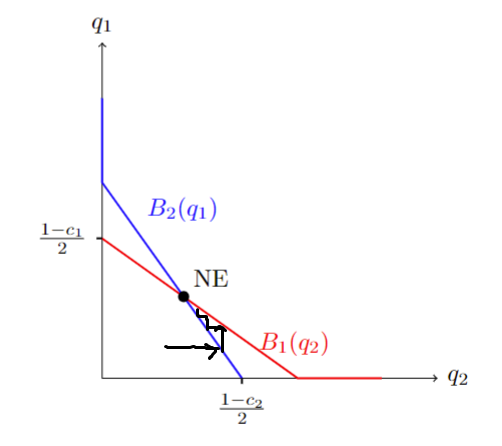
\includegraphics{cournot convergence.png}
    \end{center}
\end{aexample}
However, if we swap 
\begin{center}
    
\begin{tikzpicture}[scale=4, every node/.style={font=\small}]
    % Axes
    \draw[->] (0,0) -- (1.2,0) node[right] {$q_2$};
    \draw[->] (0,0) -- (0,1.2) node[above] {$q_1$};
    
    % Best response lines
    \draw[red, thick] (0,0.7) -- (0.5,0) node[pos=0.75, below left] {$B_1(q_2)$} -- (1,0);
    \draw[blue, thick] (0.7,0) -- (0,0.5) node[pos=0.75, above right] {$B_2(q_1)$}--(0,1);

    % Nash equilibrium point
    \fill (0.291667,0.291667) circle (0.02) node[above right] {NE};

    % Labels on axes
    \draw[thick] (0,0.7) -- (-0.02,0.7) node[left] {$\frac{1-c_1}{2}$};
    \draw[thick] (0.7,0) -- (0.7,-0.02) node[below] {$\frac{1-c_2}{2}$};
\end{tikzpicture}

\end{center}
The middle nash equilibrium point becomes unstable and the ends become stable.

\definition{Stable and unstable equilibria}{
    We call the equilibrium stable best response dynamic converges to the equilibrium and unstable otherwise.
}
\definition{Strategic complements}{
    This refers to a game where the value of a given action increases as other agents take that action.
}
\begin{aexample}{Language game}{}
    We have $N$ people and two languages, French and English. The payoff of choosing a language is equal to the number of people choosing the language. 
\end{aexample}


\begin{aexample}{Power control}{}
    There are $2$ transmitters. Each transmitter chooses the power level $P_i\in[0,1]$. The payoff function \[
    \pi_i(P_i,P_{-i}) = \begin{cases}
        1-cP_i, &\textrm{if $\frac{P_i}{P_{-i}+N}>\gamma$}\\
        0, &\textrm{otherwise}.
    \end{cases}
    \]With $c$ chosen to be small enough that it is interesting.
\end{aexample}

\definition{Increasing differences}{
    Let $X\subseteq \reals$, and $T$ a partially ordered set. Then $f:X\times T\to \reals$ has \textbf{increasing differences} if $
    \forall x'\geq x, t'\geq t   
    $\[
    f(x',t')-f(x,t')\geq f(x,t)-f(x,t).
    \]
}
\begin{remark}
    If $T\subseteq \reals^k$ (partial order is $\geq$ in every entry of the vector) and $f$ is $C^2$, this condition is equivalent to \[
        \frac{\partial^2 f}{\partial x \partial t_i}\geq 0
    \]
    for all $x$, $t_i$.
\end{remark}

\theorem{Topkis}{
    Let $X\subseteq \reals$ compact and $T$ partially ordered. Let $f:X\times T\to \reals$ be continuous in $X$ and has increasing differences. Then \begin{itemize}
        \item $x(t) \defeq \arg\max_{x\in X} f(x,t)$ is non-empty.
        \item $x(t)$ has a largest and smallest element $\bar{x}(t)$ and $\underline{x}(t)$ respectively.
        \item  $\bar{x}(t)$ and $\underline{x}(t)$ are increasing in $t$.
    \end{itemize} 
}
\begin{proof}
    The first two statements are a consequence of continuity and compactness, and the extreme value theorem.
    The last statement probably uses some kind of measure theory.
\end{proof}

\definition{Super Modularity}{
    A game $G=\{R,\{S_r\},\{\pi_r\}\}$ is \textbf{supermodular} if for all $r\in R$,\begin{itemize}
        \item $S_r$ is a compact subset of $\reals$.
        \item $\pi_r$ is continuous in $s_i$ and $s_{-i}$
        \item $\pi_r$ has increasing differences in $s_i,\bar{s}_{-i}$.
    \end{itemize}

}
\begin{remark}
    This is not the most general definition. But this is good enough.
\end{remark}
Given a supermodular game, we get that the best response $B_i\defeq \arg\max_{s_i\in S_i}\pi_i(s_i,\bar{s}_{-i})$ is non empty, has a largest and smallest element $\bar{B}_i$, $\underline{B}_i$, and these are increasing in $\bar{s}_{-i}$.
This captures the idea of complementarity. If other agents increase their strategies, the best response is to also increase. 

\begin{aexample}{}{}
    Let $s^0=(s_1^0,\ldots, s_R^0)$ where $s_i^0$ is the largest element in $S_i$. Starting here, we run parallel best response using $\bar{B}_i$ for all $i$. We show that this converges to a Nash equilibrium.
\end{aexample}
\begin{proof}
    We show that $s^k\leq s^{k-1}$ for all $k$. Then, by MCT, this converges to a Nash equilibrium. To show this, we proceed by induction. 
    The case $s^1\leq s^0$ is trivial by the definition of $s^0$.
    Then if $s^{k-1}\leq s^k$, then \[
    s_i^{k+1}=\bar{B}_i(s^k_{-i}) \leq \bar{B}_i(s^{k-1}_{-i}) = s_i^k
    \]
    by Topkis's theorem. 
\end{proof}
\begin{remark}
    We can also start from the smallest element, then work our way up to a (possibly different) Nash equilibrium. If all the strategy sets are intervals, we can consider the box that has the two vertices with the two Nash equilibria. It is not hard to see that any other Nash equilibrium has to be inside the box, by the increasing difference property. Hence, if the two equilibria are the same there is a unique equilibria.
\end{remark}
\begin{aexample}{Betrand Competition}{}
    We have $N$ firms, each firm chooses their price $p_i$. The demand for firm $i$ is \[
    D_i (p_i,\bar{p}_{-i})=a_i-b_ip_i+\sum_{j\neq i} d_{ij} p_j,
    \]where $a_i,b_i,d_{ij}\geq 0$.
    The payoff of the firm is \[
    \pi_i(p_i,\bar{p}_{-i})=p_iD_i(p_i,\bar{p}_{-i}).
    \]
    Then we have \begin{align*}
    \frac{\partial \pi_i}{\partial p_i} &= a_i-2b_ip_i+\sum_{j\neq i} d_{ij} p_j,\\
    \frac{\partial \pi_i}{\partial p_i\partial p_j} &= d_{ij} \geq 0.
    \end{align*}
    Subject to some technicalities on the prices the firms can choose, this is a supermodular game. 
\end{aexample}